%        File: 
%     Created: pon mar 29 10:00  2010 C
% Last Change: pon mar 29 10:00  2010 C
%
\documentclass[a4paper]{article}
\usepackage[]{polski}
\usepackage[utf8]{inputenc}
\usepackage[dvips]{graphicx}
\usepackage{float}
\usepackage{tikz}
\usepackage[a4paper, left=1.2cm, right=1.2cm, top=1.2cm, bottom=1cm, headsep=1.2cm]{geometry} 
\usepackage{color}
% \pagestyle{plain}
\pagestyle{empty}


\definecolor{nokiaBlue}{RGB}{18,65,145}

\newcommand*{\thickhrulefill}{%
\color{nokiaBlue}
\leavevmode % ensure horizontal mode
\leaders\hrule depth -2pt height 3pt \hfill
\kern 0pt\relax % or \kern\z@
\color{black}
} 

\newcommand*{\thickhrule}{%
\color{nokiaBlue}
\rule[2pt]{0.7cm}{1pt}
\color{black}
} 

\def\cvsekcja#1{%
\vspace{0.1cm}
\noindent\thickhrule
\MakeUppercase{\textbf{\footnotesize#1}}
\hspace{0.1cm}\color{nokiaBlue}\thickhrulefill
}

\def\cvwpis#1#2{%
%\vspace{2pt}
\noindent
\newline
\begin{minipage}[t]{0.2\textwidth}
  \begin{flushleft}
  #1 
\end{flushleft}
\end{minipage}
\begin{minipage}[t]{0.8\textwidth}
  #2
\end{minipage}
}

\def\labelitemi{--}
\usepackage{enumitem}
\setlist{nolistsep}

\begin{document}

\begin{center}
  \large{\textsc{Curriculum Vitae}\\
  Sławomir Andrzejewski}
\end{center}


\hfill
\begin{minipage}[b]{3.1cm}
  \vspace{-2.5cm}
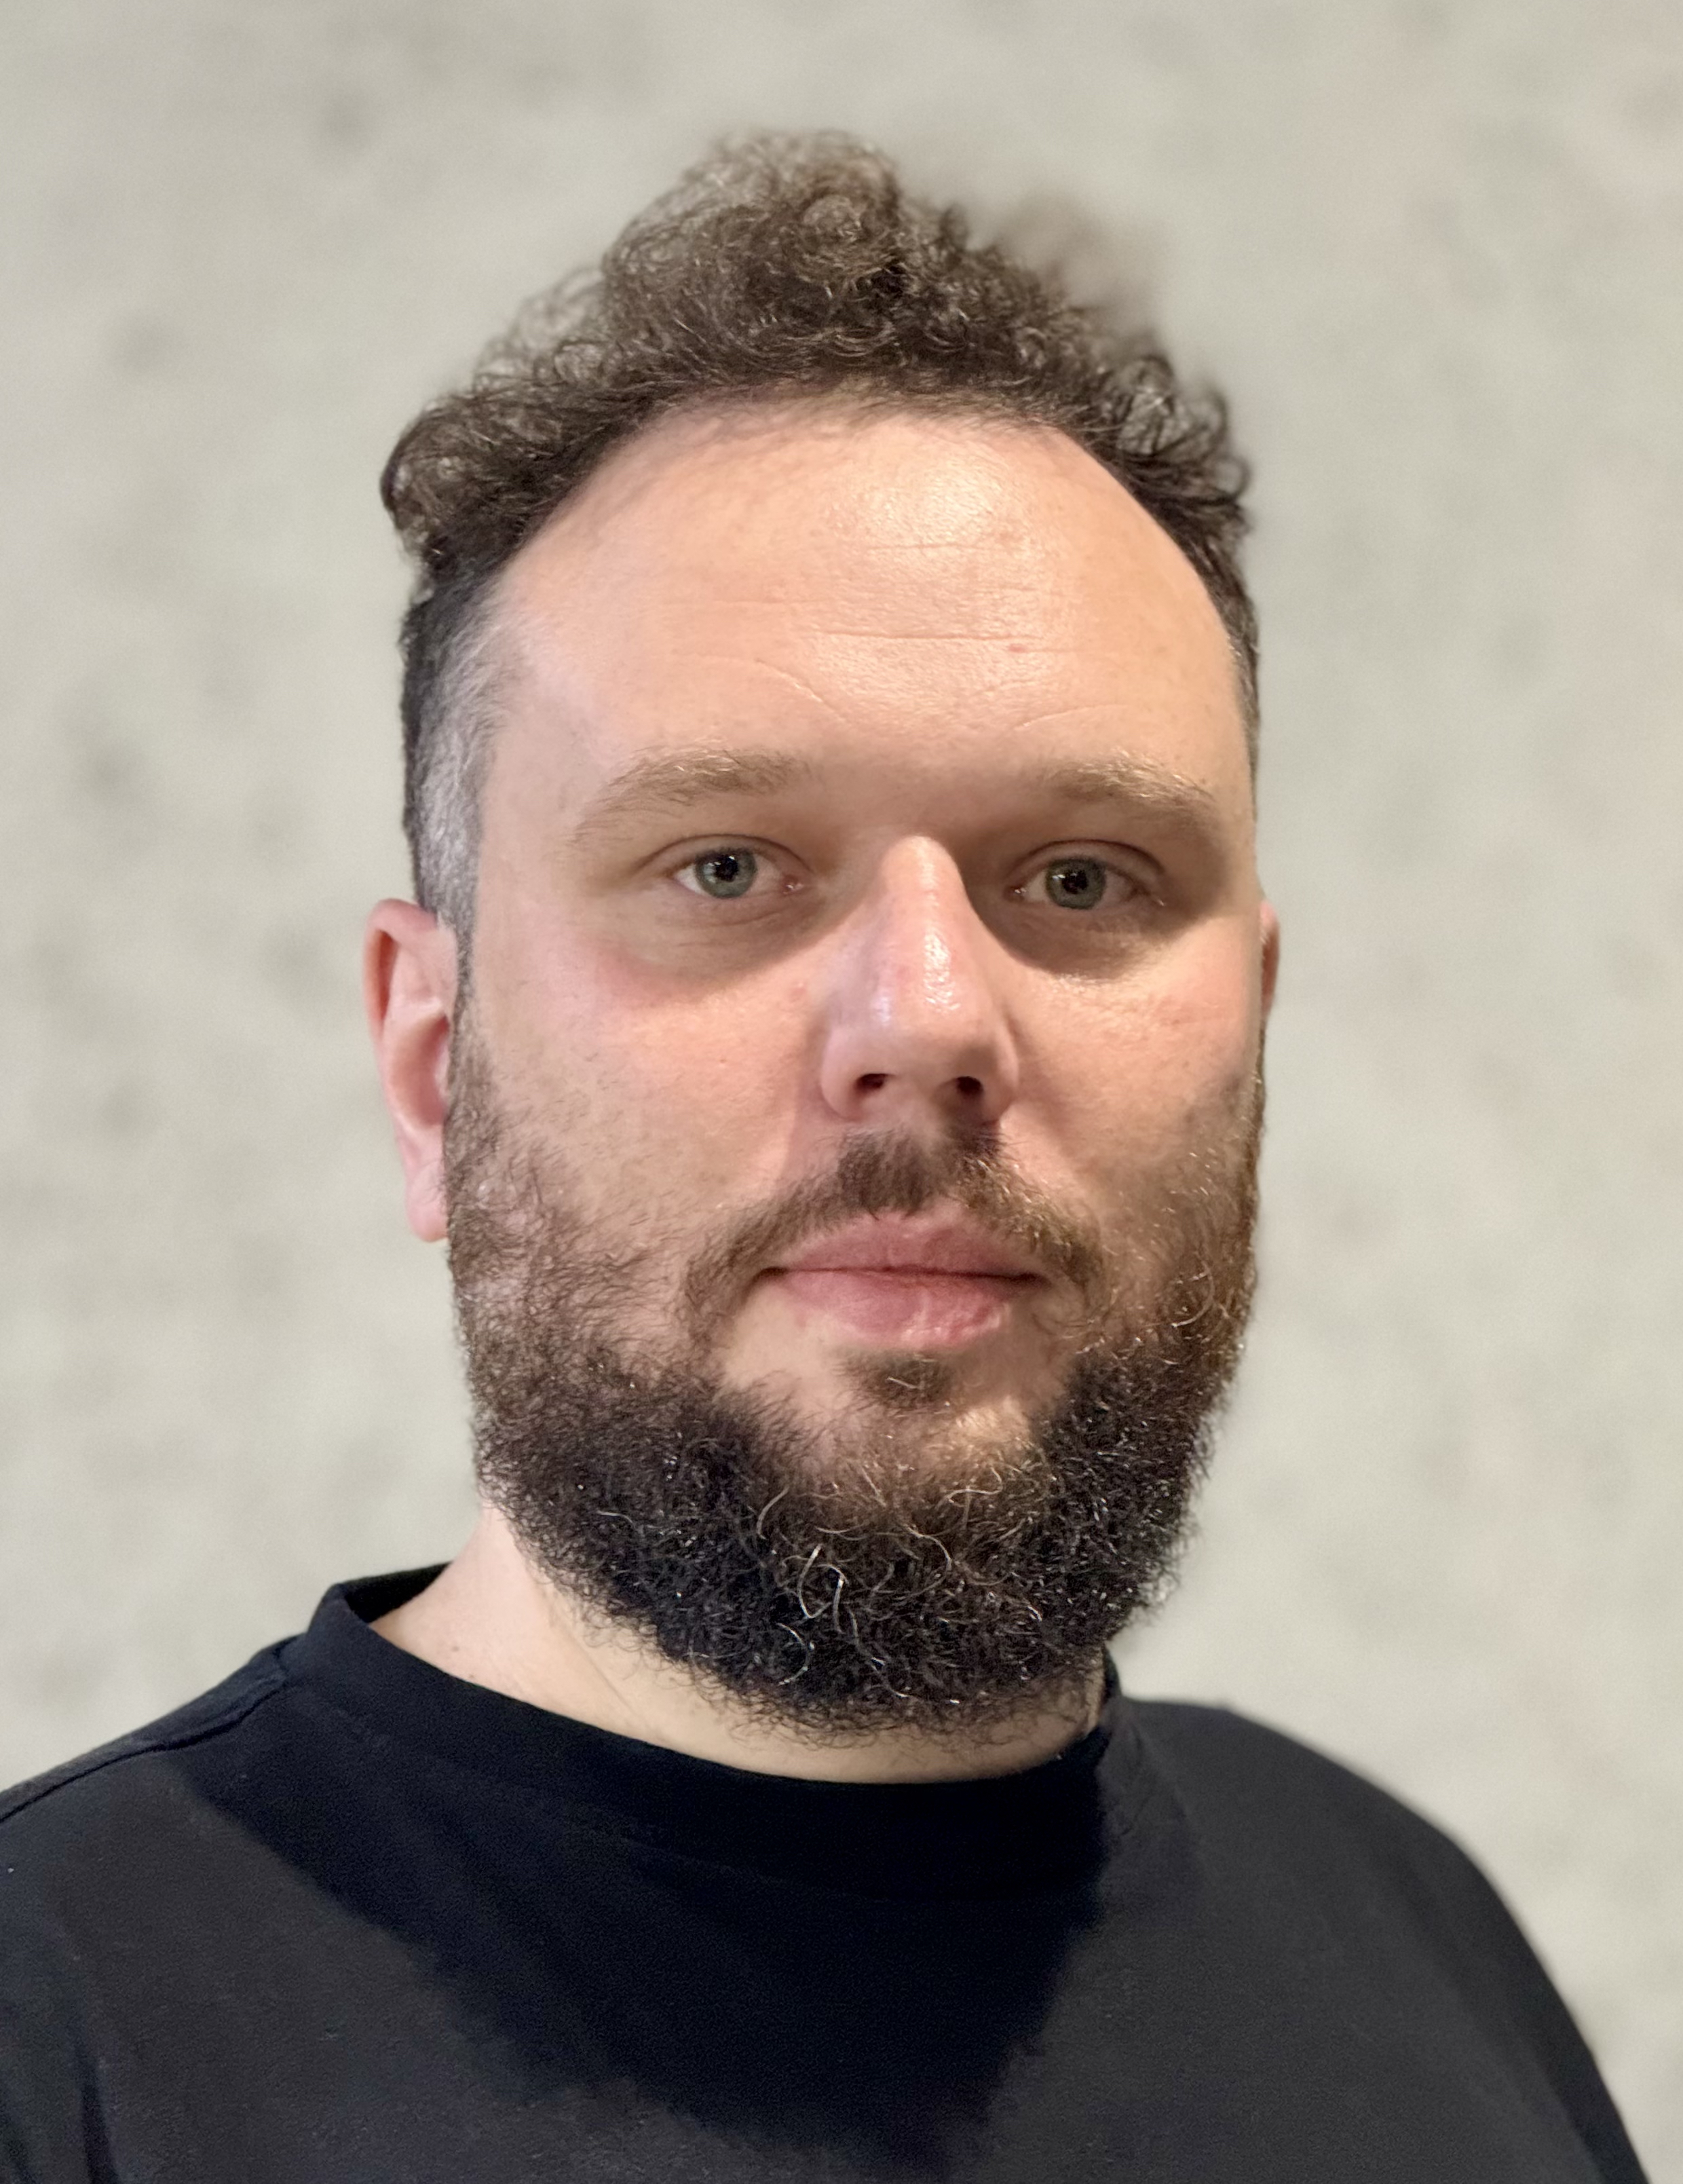
\includegraphics[width=3cm]{zdjecie}
\end{minipage}

%\cvsekcja{Personal information}
\cvsekcja{Contact}

\cvwpis{Mobile}{+48 600 465 564}
\cvwpis{E\dywiz mail}{s.j.andrzejewski@gmail.com}

%\cvwpis{Date of birth}{30th June, 1988}  
%\cvwpis{Address}{Przestrzenna 4/11\\ 50-533 Wrocław}
%\cvwpis{Mobile}{+48 784 631 874 / +48 600 465 564}
%\cvwpis{E\dywiz mail}{slawomir.andrzejewski@nsn.com / s.j.andrzejewski@gmail.com}


% ======================================== 
% EDUCATION
% ======================================== 
\cvsekcja{Education}

\cvwpis{2011 - 2012}
{Master degree:\\
Wrocław University of Technology, Faculty of Electronics\\
Major: Teleinformatics, Specialization: Teleinformation Networks Design}

\cvwpis{2007 - 2011}
{ Bachelor degree:\\
Wrocław University of Technology, Faculty of Electronics\\
Major: Teleinformatics}

% ======================================== 
% PROFESSIONAL EXPERIENCE
% ======================================== 
\cvsekcja{Professional Experience}

\cvwpis{2021 - present}
{Vonage\\
Vonage Contact Center\\
Engineering Manager\\
\vspace{-7pt}
\\Managing team of Software Developers (front-end: Type Script, React, Vue.js; back-end: .NET) and QAs.
Domain ownership (User Management, Agent Workspace), including execution and technical aspects.
Setting goals and targets, employees recruitment and evaluation. 
}

\cvwpis{2017 - 2021}
{Nokia\\
Network Engineering\\
R\&D Line Manager\\
\vspace{-7pt}
\\Managing two teams: Data Analysts and Software Engineers (mathematicians, software developers, telecommunication engineers).
Leading and supervising data-related projects.
Shaping department strategy (around 150 people), setting goals and targets.
Employees recruitment and evaluation. 
}

\cvwpis{2015 - 2017}
{Nokia\\
Network Engineering\\
Customer Support Specialist\\
\vspace{-7pt}
\\Team Leader of data engineers/analytics team. Data analytics and data mining methodologies development and
application. Projects results reporting for internal and external
customers. Tasks assignment. Team building and employees recruitment.
}

\cvwpis{2010 - 2014}
{Nokia / NSN\\
WCDMA Integration \& Verification\\
Base Station Software Integration Engineer\\
\vspace{-7pt}
\\Regression test automation.
Setup and maintenance of test environment (including automated management).
Team processes creation and update.
Employees recruitment.
}

\cvwpis{2009 - 2010}
{Wrocław University of Technology\\
\vspace{-7pt}
\\Participation in a government-sponsored research project\\
Analysis of results of simulations and statistical analysis of the
properties of a~radio channel inside buildings and a reverberation chamber.
}
\pagebreak


% ======================================== 
% SELECTED PROJECTS
% ======================================== 
\cvsekcja{Selected Projects}

\cvwpis{BTS Clustering  \vspace{5pt} \\2020 - \textit{2023}}
{
    Role: Project Leader\\
    \vspace{-8pt}
    \\Responsibilities: end-to-end responsibility; project scope definition,
        submission preparation, execution. Project management for couple of teams,
        60 people in peak.\\
    \vspace{-8pt}
    \\About the project: research project for finding and modeling the configuration-to-performance
    relationship of telecommunication network. 
        Total project cost around 5.5 M EUR; European Union grant: 50\% of
        expenses.
        Project reference number: POIR.01.01.01-00-1329/20.
}


\cvwpis{Network\\ development\\ assistant \vspace{5pt} \\2018 - 2020}
{
    Role: Project Leader\\
    \vspace{-8pt}
    \\Responsibilities: end-to-end responsibility; project scope definition,
        submission preparation, execution. Project management for couple of teams,
        60 people in peak.\\
    \vspace{-8pt}
    \\About the project: research project for automated insights generation about Nokia
        product usage and deployments. Profiling of Nokia's customers (both
        technical and business strategy).
        Total project cost around 3.5 M EUR; European Union grant: 50\% of
        expenses.
        Project reference number: POIR.01.01.01-00-1009/17.\\
    \vspace{-8pt}
    \\Personal recognition: Best in Global Services Customer Support Certificate
}

\cvwpis{webNEI app \vspace{5pt} \\ 2015 - 2017}{
    Role: Product Owner\\
    \vspace{-8pt}
    \\Responsibilities: requirements definition, tasks prioritization and
    backlog maintenance. Quality assurance, process setup.
    Managing two teams (one local, one remote), 12 people in peak.\\
    \vspace{-8pt}
    \\About the project: creating web-based application for technical
    documents life-cycle management and sharing. App has been productized -
    around 17k unique users.
}

% ======================================== 
% PUBLICATIONS
% ======================================== 
\cvsekcja{Articles and publications}

\cvwpis{2016}{Nokia Book, 2nd edition: Shaping the future of telecommunication\\'Big-data-driven Telco Market'}
\cvwpis{2014}{Software Developer's Journal\\'About source code revision systems - Subversion'}
\cvwpis{2013}{Programista Magazine\\ ‘Automated acceptance testing in continuous delivery process’}

% ======================================== 
% COURSES AND TRAININGS
% ======================================== 
\cvsekcja{Trainings and Certifications}

\cvwpis{2018}{SAFe 4 Agilist Certificate}
\cvwpis{2012}{ISTQB Tester Foundation Level Certification}
\cvwpis{2009-2010}{CISCO CCNA Exploration:\\
    Network Fundamentals;
    Routing Protocols and Concepts;
    LAN Switching and Wireless}

% ======================================== 
% SKILLS and QUALIFICATIONS
% ======================================== 
\cvsekcja{Skills and Qualifications}

\cvwpis{Languages} {Polish: native, English: advanced}
\vspace{5pt}
\cvwpis{Project management}{
    Scaled Agile Framework (SAFe), Scrum, Kanban\\
    Tooling: JIRA (including administration), Confluence, Slack, MS Teams}
\vspace{5pt}
\cvwpis{Software and data}{
    Strong understanding of software development processes and methodologies\\
    Python, Git \\
    Software architecture, message brokers \\
    Microservices \\
    Understanding of (big) data processing (SQL and non-SQL databases, Hadoop) \\
    Understanding of Machine Learning techniques}
\vspace{5pt}
\cvwpis{Telecommunication} {5G, LTE, WCDMA, radio waves propagation}
\vspace{5pt}


\vfill
\color{gray}
\begin{center} \tiny{
    I hereby give my permission to process my personal data as included in my offer
    (under the act from 29.08.1997 regarding Personal Data Protection; uniform text: Dz. U. z 2002r. Nr 101, 
    poz. 926 ze zm.).}
\end{center}

\end{document}
